% !TeX program = pdflatex
\documentclass[journal]{IEEEtran}
\usepackage[T1]{fontenc}
\usepackage[utf8]{inputenc}
\usepackage{amsmath,amssymb}
\usepackage{array}
\usepackage{booktabs}
\usepackage{graphicx}
\usepackage{multirow}
\usepackage{url}
\usepackage{xcolor}
\usepackage{placeins}
\graphicspath{{../figures/}{./}}
\hyphenation{crowd-sens-ing block-chain rep-u-ta-tion}

\begin{document}
\title{Supplementary Material for RQ3:\ Worker-Side Poisoning Robustness of IRPP-TD}
\author{Anonymous Authors}
\maketitle

\section{Evaluation Contract and Trust Boundary}
\label{app:rq3-contract}

This supplement records the complete RQ3 contract behind Fig.~3 in the main
experimental section. RQ3 tests a worker-side adversary that can coordinate
ordinary worker reports and time its behavior using public task progress. The
adversary does not control the data requester, reputation blockchain, or trusted
bootstrap source. The $s_0=5$ bootstrap workers (IDs 1001--1005) are
platform-affiliated workers with aligned incentives and are assumed fully
honest. Their corruption is outside the worker-side adversarial model considered
in RQ3; no result below should be read as robustness to a compromised bootstrap
source.

The test reuses the RQ1 Climate, Traffic, and Water task incidence generated by
the stored SUMO trajectories. The primary workload has target participation
$\bar n=27$, and $\bar n=39$ is a replication. Worker IDs remain 1--100 and
each workload contains 100 tasks. Tasks 1--20 retain their calibration role;
accuracy is evaluated on tasks 21--100, except that attack-mode outcomes are
restricted to the blocks in which the corresponding attack is active. Table~
\ref{tab:rq3-settings} gives the complete fixed configuration.

\begin{table*}[!t]
\centering
\caption{Complete RQ3 Configuration}
\label{tab:rq3-settings}
\scriptsize
\setlength{\tabcolsep}{4.2pt}
\renewcommand{\arraystretch}{1.09}
\begin{tabular}{p{0.18\textwidth}p{0.76\textwidth}}
\toprule
Item & Fixed setting \\
\midrule
Workloads & Climate, Traffic, and Water; 100 tasks; target $\bar n=27$ in the main test and $\bar n=39$ for replication; original SUMO incidence retained. \\
Ordinary workers & IDs 1--100; malicious sets are activity-balanced, nested within each workload and seed, and contain $\operatorname{round}(100\rho_m)$ IDs. \\
Trusted bootstrap & IDs 1001--1005; honest, disjoint from ordinary workers, and supplied adaptively only while fewer than $n_b=5$ mature ordinary anchors exist. \\
Randomness & 30 paired seeds, 20260808--20260837; the same task incidence, honest report, malicious membership, attack report, and attack direction are replayed across compared methods. \\
Prevalence and strength & $\rho_m\in\{0,0.1,\ldots,0.8\}$ and $\kappa\in\{0.1,0.25,0.5,1,2\}$; the primary attack point is $(\rho_m,\kappa)=(0.3,0.5)$. \\
Schedules & Immediate attacks begin at task 1; On--Off attacks are active on 21--30, 41--50, 61--70, and 81--90; Mature-Anchor attackers behave honestly through task 40 and poison from task 41 onward. \\
Frozen IRPP-TD & $\zeta=0.25$, $\theta=0.35$, $\mu_1=0.05822585$, $\mu_2=0.00172272$, $e_b=n_b=s_0=5$, $q_b=2$, $\delta_{\max}=20$, $\epsilon_d=\epsilon_w=10^{-12}$, TD $\epsilon=10^{-5}$, and $t_{\max}=50$. \\
Screening thresholds & IRPP-TD uses its frozen RABOD decision and RPPS-TDC keeps the retained source threshold $p=0.3$. PRTD has no hard-rejection output, so its effective-weight gate is selected on a separate clean replay, tasks 1--20, to 96\% clean acceptance and then frozen. No attack outcome tunes any threshold. \\
Statistics & Scene-macro point estimates; 2,000 paired-seed bootstrap repetitions for 95\% intervals. No RQ3 outcome is used to retune a parameter. \\
Operational failure & $R_E\geq5$ or no-truth rate above 5\%, where $R_E$ is attacked NRMSE divided by the phase-matched clean NRMSE. This is an empirical operating criterion, not a theoretical breakdown point. \\
\bottomrule
\end{tabular}
\end{table*}

\section{Controlled Report and Attack Construction}
\label{app:rq3-attacks}

Let $\mathbf y_t$ be the task reference and let $\mathbf c$ and $\mathbf s$
be the coordinate-wise center and $Q_{0.95}-Q_{0.05}$ scale fitted only to the
RQ1 calibration partition. An honest coordinate is drawn from a zero-mean
Gaussian with standard deviation $0.01|y_{t,j}|/3$ and clipped between
$\min(0.99y_{t,j},1.01y_{t,j})$ and
$\max(0.99y_{t,j},1.01y_{t,j})$. We write
$\mathbf z=(\mathbf d-\mathbf c)/\mathbf s$ for the normalized report. Every
active attack satisfies, up to the stated compact jitter,
\begin{equation}
 \frac{1}{\sqrt{\ell}}
 \left\|\frac{\mathbf d^{\rm atk}-\mathbf d^{\rm hon}}{\mathbf s}\right\|_2
 =\kappa .
 \label{eq:rq3-strength}
\end{equation}

\textit{Independent bias:}
Each active malicious worker draws a deterministic seed-paired Rademacher
direction $\mathbf u_{i,t}\in\{-1,+1\}^{\ell}$ and submits
$\mathbf z^{\rm atk}_{i,t}=\mathbf z^{\rm hon}_{i,t}+\kappa\mathbf u_{i,t}$.

\textit{Compact collusion:}
The coalition computes the coordinate-wise median $\widetilde{\mathbf z}_t$ of
its own benign observations and submits reports around
$\widetilde{\mathbf z}_t+\kappa\mathbf v_1$, where $\mathbf v_1$ is the first
principal direction from calibration reports and
$\|\mathbf v_1\|_2=\sqrt{\ell}$. Independent Gaussian jitter has standard
deviation $0.02\kappa$. Thus, the attack is compact and coordinated but its
target does not read the task reference.

\textit{On--Off and Mature-Anchor poisoning:}
Both use the compact report when active. On--Off alternates the four active
blocks in Table~\ref{tab:rq3-settings} with benign blocks. Mature-Anchor behaves
honestly for 40 tasks so that coalition members can enter the reputation-guided
reference, then switches permanently at task 41. The latter directly probes the
reviewer-identified feedback loop rather than corrupting the trusted HQ5.

\section{Compared Implementations and Metrics}
\label{app:rq3-fairness}

IRPP-TD, CRH-N, PRTD, QE, and RPPS-TDC receive byte-identical ordinary reports
for a given replay. Panels (a) and (b) use the unchanged RQ1 aggregation
adapters and parameters. Fig.~3(c) compares method-faithful hard decisions:
IRPP-TD uses its native RABOD label, RPPS-TDC uses its native sequential
quality rule at $p=0.3$, and PRTD screens by its final effective weight
$n\gamma_i\omega_i/\sum_j\gamma_j\omega_j$ at the clean fourth-percentile
gate, then reruns the unchanged aggregation on retained reports. Clean
calibration is repeated inside each paired workload--seed replay, so its
variation enters the reported intervals. CRH-N and PRTD otherwise operate in
their native representation, and no task reference enters an aggregation
update. IRPP-TD additionally invokes its declared adaptive HQ5 bootstrap
mechanism. This is a system-level comparison rather than an equal-report-cost
comparison; RQ2 separately quantifies the bootstrap report cost.

The primary metric is returned-task NRMSE. No-truth is reported separately and
is never silently removed from the denominator of its rate. Malicious-report
leakage is the fraction of active malicious reports retained by IRPP-TD's
native RABOD decision, RPPS-TDC's native $p=0.3$ decision, or PRTD's
clean-calibrated relative-weight gate. Honest-report acceptance reports the
corresponding collateral cost. CRH-N has no report-selection output; QE's
exhaustive local-support scan remains in the accuracy comparison but is not
treated as the reputation-threshold filter in Fig.~3(c). Honest false-low is
the fraction of noncoalition reports assigned
the low-quality label. Ordinary-anchor purity excludes HQ5 and treats a
coalition member as malicious even during its reputation-building phase. This
definition makes the latent feedback risk visible before the task-41 switch.

\section{Complete RQ3 Results}
\label{app:rq3-results}

The following figure and tables report the replication, operating-boundary,
and clean-calibrated baseline evidence underlying the main-text panels.

\begin{figure*}[!t]
\centering
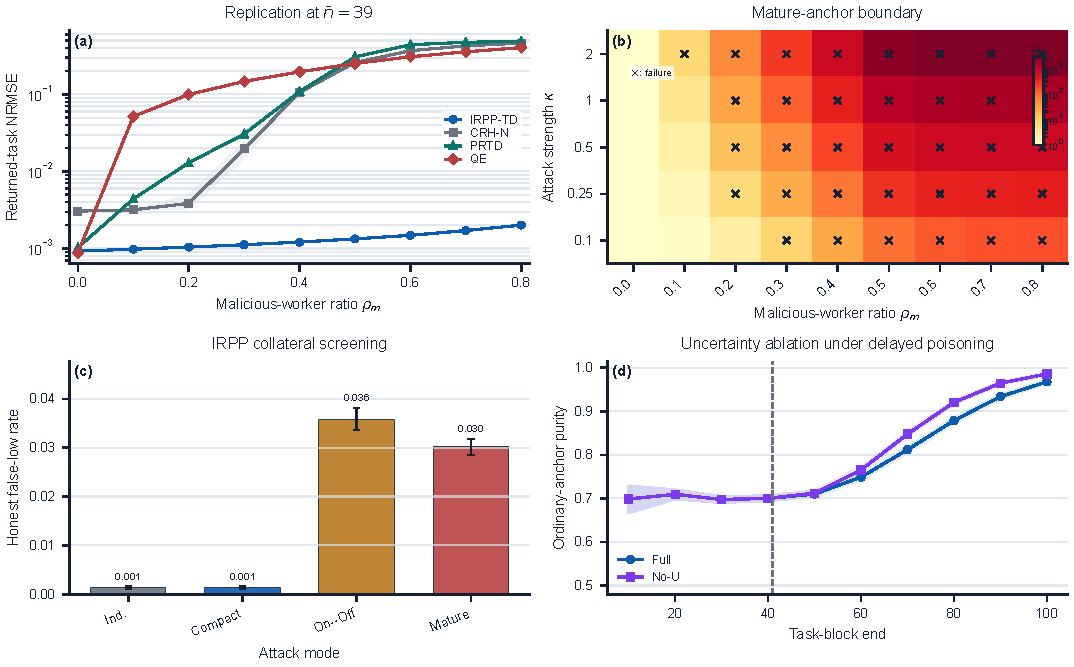
\includegraphics[width=0.95\textwidth]{fig_rq3_supplement_2x2.pdf}
\caption{Worker-level and replication evidence complementary to main-text
Fig.~3. (a) Compact-collusion prevalence at $\bar n=39$. (b) Mature-Anchor
error ratio over the complete prevalence--strength grid; crosses mark the
operational criterion. (c) IRPP-TD honest false-low rate across attack modes at
$(\rho_m,\kappa)=(0.3,0.5)$. (d) Full and No-U ordinary-anchor purity under
task-41 Mature-Anchor poisoning. Bars and bands carry 95\% paired-seed
bootstrap intervals.}
\label{fig:rq3-supplement}
\end{figure*}

\begin{table*}[!t]
\centering
\caption{Active-Task NRMSE Across Clean and Attack-Mode Replays at
$\bar n=27$}
\label{tab:rq3-mode-methods}
\scriptsize
\setlength{\tabcolsep}{8.0pt}
\renewcommand{\arraystretch}{1.05}
\begin{tabular}{lrrrrr}
\toprule
Method & Clean & Independent & Compact & On--Off & Mature-Anchor \\
\midrule
IRPP-TD & 0.00113 & 0.00137 & 0.00137 & 0.03631 & 0.03315 \\
CRH-N   & 0.00341 & 0.09963 & 0.04045 & 0.03544 & 0.04094 \\
PRTD    & 0.00127 & 0.00886 & 0.04634 & 0.04213 & 0.04430 \\
QE      & 0.00107 & 0.05216 & 0.14769 & 0.14883 & 0.14866 \\
\bottomrule
\end{tabular}
\par\vspace{0.4ex}
\parbox{0.91\textwidth}{\scriptsize Attack replays use
$(\rho_m,\kappa)=(0.3,0.5)$; Clean uses $\rho_m=0$. Each attack is evaluated
only on its active task set. Fig.~3(b) reports the corresponding 95\%
paired-seed bootstrap intervals.}
\end{table*}

\begin{table*}[!t]
\centering
\caption{Primary and Boundary RQ3 Outcomes}
\label{tab:rq3-complete}
\scriptsize
\textbf{(a) Compact-collusion prevalence: scene-macro NRMSE}\par\vspace{0.35ex}
\setlength{\tabcolsep}{4.0pt}
\begin{tabular}{ccrrrr}
\toprule
$\bar n$ & $\rho_m$ & IRPP-TD & CRH-N & PRTD & QE \\
\midrule
27 & 0.0 & 0.00113$\pm$0.00001 & 0.00341$\pm$0.00002 & 0.00127$\pm$0.00001 & 0.00107$\pm$0.00001 \\
27 & 0.3 & 0.00137$\pm$0.00002 & 0.0404$\pm$0.0036 & 0.0463$\pm$0.0038 & 0.148$\pm$0.001 \\
27 & 0.5 & 0.00164$\pm$0.00002 & 0.270$\pm$0.005 & 0.313$\pm$0.003 & 0.254$\pm$0.000 \\
27 & 0.8 & 0.00215$\pm$0.00002 & 0.465$\pm$0.001 & 0.488$\pm$0.000 & 0.406$\pm$0.000 \\
\midrule
39 & 0.0 & 0.00093$\pm$0.00001 & 0.00305$\pm$0.00003 & 0.00102$\pm$0.00001 & 0.00088$\pm$0.00001 \\
39 & 0.3 & 0.00112$\pm$0.00001 & 0.0196$\pm$0.0050 & 0.0305$\pm$0.0022 & 0.147$\pm$0.000 \\
39 & 0.5 & 0.00133$\pm$0.00001 & 0.259$\pm$0.004 & 0.306$\pm$0.003 & 0.252$\pm$0.001 \\
39 & 0.8 & 0.00201$\pm$0.00003 & 0.464$\pm$0.001 & 0.488$\pm$0.000 & 0.404$\pm$0.000 \\
\bottomrule
\end{tabular}
\par\vspace{1.1ex}
\begin{minipage}[t]{0.31\textwidth}
\centering\textbf{(b) Mature-anchor operational boundary}\par\vspace{0.35ex}
\setlength{\tabcolsep}{3.2pt}\begin{tabular}{rrrr}
\toprule $\kappa$ & Fail $\rho_m$ & $R_E@.8$ & Max NT (\%) \\
\midrule 0.1&0.3&141.05&0.02\\ 0.25&0.2&354.65&0.15\\ 0.5&0.2&710.72&0.22\\ 1&0.2&1422.11&0.13\\ 2&0.1&2844.40&0.19\\
\bottomrule\end{tabular}
\end{minipage}\hfill
\begin{minipage}[t]{0.31\textwidth}
\centering\textbf{(c) Malicious-report leakage}\par\vspace{0.35ex}
\setlength{\tabcolsep}{3.0pt}\begin{tabular}{lrrr}
\toprule Mode & IRPP-TD & RPPS-TDC & PRTD \\
\midrule Independent&0.000&0.00025&0.719\\ Compact&0.000&0.080&0.777\\ On--Off&0.249&0.293&0.780\\ Mature&0.206&0.295&0.779\\
\bottomrule\end{tabular}
\end{minipage}\hfill
\begin{minipage}[t]{0.31\textwidth}
\centering\textbf{(d) Ordinary-anchor purity}\par\vspace{0.35ex}
\setlength{\tabcolsep}{3.2pt}\begin{tabular}{lrrr}
\toprule Variant & B40 & B50 & B100 \\
\midrule Full&0.700&0.710&0.968\\ Binary-Rep.&0.700&0.711&0.984\\ No-U&0.700&0.712&0.986\\ All-Anchors&0.699&0.699&0.697\\ Sequential&0.699&0.699&0.697\\
\bottomrule\end{tabular}
\end{minipage}
\par\vspace{0.4ex}
\parbox{0.97\textwidth}{\scriptsize Panel (a) reports means $\pm$ the larger
95\% paired-seed bootstrap half-width. Failure in (b) means $R_E\geq5$ or
no-truth above 5\%. Thresholds in (c) are fixed before attack evaluation;
only PRTD's added gate is fitted on clean tasks 1--20.}
\end{table*}

\newpage

Table~\ref{tab:rq3-complete}(a) and Fig.~\ref{fig:rq3-supplement}(a)
show that the immediate compact-collusion conclusion replicates at the larger
participation level. At $\bar n=27$ and
$\rho_m=0.8$, IRPP-TD has 0.00215 NRMSE, whereas CRH-N, PRTD, and QE have
0.465, 0.488, and 0.406. The prevalence sweep has zero no-truth outcomes for
all four methods.

Table~\ref{tab:rq3-mode-methods} complements the prevalence sweep with matched
algorithm comparisons across attack schedules. IRPP-TD is lowest under both
immediate modes, with 0.00137 NRMSE versus 0.00886 for the closest Independent
baseline and 0.04045 for the closest Compact baseline. QE is marginally lower
on clean data, at 0.00107 versus 0.00113. Under On--Off, CRH-N and IRPP-TD give
0.03544 and 0.03631; under Mature-Anchor, IRPP-TD is lowest at 0.03315.
Thus, reputation-aware timing narrows the immediate-attack advantage without
overturning IRPP-TD's unique near-clean result across both immediate geometries.

The delayed grid in Table~\ref{tab:rq3-complete}(b) exposes a different operating
regime. Mature attackers cross the $R_E=5$ criterion at smaller prevalence as
$\kappa$ increases. No-truth remains below 0.23\% in every cell; hence these
failures reflect inaccurate returned aggregates, not widespread abstention.
The full surface is shown in Fig.~\ref{fig:rq3-supplement}(b). At the primary
point, IRPP-TD fully rejects immediate Independent and Compact attacks, whereas
On--Off and Mature-Anchor reports leak after first building reputation.
IRPP-TD leakage is 0, 0, 0.249, and 0.206 across Independent, Compact, On--Off,
and Mature-Anchor. Native RPPS-TDC gives 0.00025, 0.080, 0.293, and 0.295;
its honest-report acceptance is 0.730--0.986, below IRPP-TD's 0.953--0.993.
PRTD accepts over 0.999 of honest reports but also retains 0.719--0.780 of
poison. The RPPS-TDC source threshold accepts 52.9\% of reports on the separate
clean tasks 1--20, confirming that its low immediate leakage is accompanied by
aggressive collateral filtering. IRPP-TD therefore provides the strongest
joint accuracy, poison rejection, and honest-report preservation, while timed
attackers remain a documented feedback limitation.

Table~\ref{tab:rq3-complete}(d) and Fig.~\ref{fig:rq3-supplement}(d) separate
containment from prevention. Full,
Binary-Rep., and No-U guided anchoring all remove coalition members from the
ordinary anchor set after the switch; Full purity reaches 0.968 by block 100.
All-Anchors and Sequential cannot purify that reference and remain near the
population baseline of 0.70. For Full, the phase-matched error ratio falls from
71.61 in block 50 to 54.78, 28.64, 9.23, 3.39, and 1.35 in blocks
60--100. For On--Off, inactive blocks 40, 60, 80, and 100 return to ratios
1.03, 1.05, 1.06, and 1.07, but every later active block again incurs a large error.
Thus, reputation-guided anchoring supports recovery from a permanent switch;
without explicit forgetting or change-point logic, it does not prevent repeated
bursts from exploiting stale reputation.

\section{Reproducibility and Integrity Checks}
\label{app:rq3-reproducibility}

The experiment is stored in a new directory and does not modify the legacy
IRPP source. Six formal shards each contain five seeds. The primary run records
1,044,000 task outcomes and 2,226,690 report-level decisions; the mode-wise
baseline extension adds 135,000 task outcomes, and the Mature-Anchor grid adds
405,000. The clean-calibrated QE/PRTD audit adds 414,000 task outcomes and
180 workload--seed calibration records. The RPPS-TDC extension adds 36,000
sequential task-level screening records and 90 clean-threshold measurements;
the earlier no-gate diagnostic records 720 scene--seed--method rates.
Automated checks verify all
30 seeds, unique task/report keys, finite metrics for returned truths, nested
malicious sets, honest HQ5 reports, schedule transitions, PRTD clean acceptance
within 0.95--0.97, fixed RPPS-TDC $p=0.3$, nondegenerate leakage, and the implication that
every active poison belongs to the selected coalition. The six primary and six
calibrated-extension manifests also agree on the hashes of the data generator,
model wrapper, and baseline adapters. The retained baseline source SHA-256 prefixes are
\texttt{95a89b80} (CRH-N), \texttt{e4242705} (QE), \texttt{1f5a5d63}
(PRTD), \texttt{755e7d7c} (RPPS-TDC TD), and \texttt{6d3a27c9}
(RPPS-TDC reputation); the integrity-audit JSON records the complete check.

\end{document}
